\documentclass{beamer}

\usetheme[bgphoto, nologo]{polimi}




%------------------------------------------------------------------------------
%	REQUIRED PACKAGES AND  CONFIGURATIONS
%------------------------------------------------------------------------------
% PACKAGES FOR TITLES
\usepackage{color}

% PACKAGES FOR LANGUAGE AND FONT
\usepackage[utf8]{inputenc}
\usepackage[english]{babel}
\usepackage[T1]{fontenc} % Font encoding
% PACKAGES FOR IMAGES
\usepackage{graphicx}
\graphicspath{{Images/}} % Path for images' folder
\usepackage{eso-pic} % For the background picture on the title page
\usepackage{subfig} % Numbered and caption subfigures using \subfloat
\usepackage{caption} % Coloured captions
\usepackage{transparent}

% STANDARD MATH PACKAGES
\usepackage{amsmath}
\usepackage{amsthm}
\usepackage{bm}
\usepackage[overload]{empheq}  % For braced-style systems of equations

% PACKAGES FOR TABLES
\usepackage{tabularx}
\usepackage{longtable} % tables that can span several pages
\usepackage{colortbl}

% PACKAGES FOR ALGORITHMS (PSEUDO-CODE)
\usepackage{algorithm}
\usepackage{algorithmic}

% PACKAGES FOR THE APPENDIX
\usepackage{appendix}

% PACKAGES FOR ITEMIZE & ENUMERATES

% OTHER PACKAGES
\usepackage{amsthm,thmtools,xcolor} % Coloured "Theorem"
\usepackage{comment} % Comment part of code
\usepackage{lipsum} % Insert dummy text
\usepackage{tcolorbox} % Create coloured boxes (e.g. the one for the key-words)
\usepackage{stfloats} % Correct position of the tables
\usepackage{multirow}
\usepackage{multicol}





%-------------------------------------------------------------------------
%	NEW COMMANDS DEFINED
%-------------------------------------------------------------------------
% EXAMPLES OF NEW COMMANDS -> here you see how to define new commands
\newcommand{\bea}{\begin{eqnarray}} % Shortcut for equation arrays
\newcommand{\eea}{\end{eqnarray}}
\newcommand{\e}[1]{\times 10^{#1}}  % Powers of 10 notation
\newcommand{\mathbbm}[1]{\text{\usefont{U}{bbm}{m}{n}#1}} % From mathbbm.sty
\newcommand{\pdev}[2]{\frac{\partial#1}{\partial#2}}
% NB: you can also override some existing commands with the keyword \renewcommand



% \setbeamertemplate{theorem begin}
% {%
%   \par\vskip\medskipamount%
%   \begin{beamercolorbox}[colsep*=.75ex]{block title}
%     \usebeamerfont*{block title}%
%       \inserttheoremname
%       \ifx\inserttheoremaddition\empty\else\ (\inserttheoremaddition)\fi%
%   \end{beamercolorbox}%
%   {\parskip0pt\par}%
%   \ifbeamercolorempty[bg]{block title}
%   {}
%   {\ifbeamercolorempty[bg]{block body}{}{\nointerlineskip\vskip-0.5pt}}%
%   \usebeamerfont{block body}%
%   \vskip-.25ex\vbox{}%
% }
% \setbeamertemplate{theorem end}{}




\newcommand*{\theorembreak}{\(\downarrow\)\usebeamertemplate{theorem end}\framebreak\usebeamertemplate{theorem begin}\rotatebox[origin=c]{180}{$\Lsh$}}





\makeatletter
\newenvironment<>{proofs}[1][\proofname]{%
    \par
    \def\insertproofname{#1\@addpunct{.}}%
    \usebeamertemplate{proof begin}#2}
  {\usebeamertemplate{proof end}}
\newenvironment<>{proofc}{%
  \setbeamertemplate{proof begin}{\begin{block}{}}
    \par
    \usebeamertemplate{proof begin}}
  {\usebeamertemplate{proof end}}
\newenvironment<>{proofe}{%
    \par
    \pushQED{\qed}
    \setbeamertemplate{proof begin}{\begin{block}{}}
    \usebeamertemplate{proof begin}}
  {\popQED\usebeamertemplate{proof end}}






%----------------------------------------------------------------------------
%	ADD YOUR PACKAGES (be careful of package interaction)
%----------------------------------------------------------------------------
\usepackage{amsfonts} 
\usepackage[font=footnotesize,labelfont=bf]{caption}

%----------------------------------------------------------------------------
%	ADD YOUR DEFINITIONS AND COMMANDS (be careful of existing commands)
%----------------------------------------------------------------------------
\usepackage{import}
\usepackage{xifthen}
\usepackage{pdfpages}
\usepackage{transparent}
\usepackage{wrapfig}
\usepackage{dsfont}

\parindent=0pt

\newcommand{\incfig}[1]{%
    \def\svgwidth{\columnwidth}
    \import{./figures/}{#1.pdf_tex}
}
\newcommand*{\oldepsilon}{\epsilon}
\renewcommand*{\epsilon}{\varepsilon}
\DeclareMathOperator*{\esssup}{ess\,sup}

\numberwithin{equation}{section}
%----------------------------------------------------------------------------
%	CONFIGURATION OF THEOREM ENVIRONMENTS


% \newtheoremstyle{break}
%     {\partopsep}{\topsep}%  
%     {\normalfont}{}
%     {\bfseries}{}%
%     {\newline}{}%
% \theoremstyle{break}
% \newtheorem{theorem}{Theorem}[section]
% \newtheorem{corollary}{Corollary}[section]
% \newtheorem{proposition}{Proposition}[section]
% \newtheorem{remark}{Remark}[section]
% \newtheorem{lemma}{Lemma}[section]
% \newtheorem{notation}{Notation}[section]
% \newtheorem{definition}{Definition}[section]

% \newtheorem{definition}{Definition}[section]

\newtheorem*{remark}{Remark}


\setbeamertemplate{theorems}[numbered]

% %----------------------------------------------------------------------------

% Do not change Configuration_files/config.tex file unless you really know what you are doing.
% This file ends the configuration procedures (e.g. customizing commands, definition of new commands)
% Set the geometric layout of the document
\usepackage{geometry}
\geometry{
  top=3cm,
  left = 2.0cm,
  right = 2.0cm,
  bottom=2cm,
  headheight= 2cm,
  headsep= 0cm,
}
\raggedbottom

% Create color bluePoli (-> manuale grafica coordinata:  https://www.polimi.it/fileadmin/user_upload/il_Politecnico/grafica-coordinata/2015_05_11_46xy_manuale_grafica_coordinata.pdf)
\definecolor{bluePoli}{cmyk}{0.4,0.1,0,0.4}

% Custom theorem environments
\declaretheoremstyle[
  shaded={rulecolor=bluePoli!20, rulewidth=1pt, bgcolor=bluePoli!5},
  headfont=\color{bluePoli}\normalfont\bfseries,
  bodyfont=\color{black}\normalfont,
]{colored}

\captionsetup[figure]{labelfont={color=bluePoli}} % Set colour of the captions
\captionsetup[table]{labelfont={color=bluePoli}} % Set colour of the captions
\captionsetup[algorithm]{labelfont={color=bluePoli}} % Set colour of the captions

\theoremstyle{colored}
\newtheorem{theorem}{Theorem}[section]
\newtheorem{proposition}{Proposition}[section]
\newtheorem{definition}{Definition}[section]
\newtheorem*{remark}{Remark}
\newtheorem{lemma}{Lemma}[section]

% Enhances the features of the standard "table" and "tabular" environments.
\newcommand\T{\rule{0pt}{2.6ex}}
\newcommand\B{\rule[-1.2ex]{0pt}{0pt}}

% Algorithm description
\newcounter{algsubstate}
\renewcommand{\thealgsubstate}{\alph{algsubstate}}
\newenvironment{algsubstates}{
    \setcounter{algsubstate}{0}%
    \renewcommand{\STATE}{%
    \stepcounter{algsubstate}%
    \Statex {\small\thealgsubstate:}\space}
    }{}

% Custom theorem environment
\newcolumntype{L}[1]{>{\raggedright\let\newline\\\arraybackslash\hspace{0pt}}m{#1}}
\newcolumntype{C}[1]{>{\centering\let\newline\\\arraybackslash\hspace{0pt}}m{#1}}
\newcolumntype{R}[1]{>{\raggedleft\let\newline\\\arraybackslash\hspace{0pt}}m{#1}}

% Custom itemize environment
\setlist[itemize,1]{label=$\bullet$}
\setlist[itemize,2]{label=$\circ$}
\setlist[itemize,3]{label=$-$}
\setlist{nosep}

% Set separation of columns
\setlength{\columnsep}{30pt}

% Create command for background pic
\newcommand\BackgroundPic{% Adding background picture
	\put(230,358){
		\parbox[b][\paperheight]{\paperwidth}{%
			\vfill
			\centering
			\transparent{0.2}
			
\includegraphics[width=0.8\paperwidth]{raggiera_polimi.eps}%
			\vfill
}}}

% Set indentation
%\setlength\parindent{0pt}

% Custom title commands
\titleformat{\section}
{\color{bluePoli}\normalfont\Large\bfseries}
{\color{bluePoli}\thesection.}{1em}{}
\titlespacing*{\section}
{0pt}{2ex}{1ex}

\titleformat{\subsection}
{\color{bluePoli}\normalfont\large\bfseries}
{\color{bluePoli}\thesubsection.}{1em}{}
\titlespacing*{\subsection}
{0pt}{2ex}{1ex}

\titleformat{\subsubsection}
{\color{bluePoli}\normalfont\normalsize\bfseries}
{\color{bluePoli}\thesubsubsection.}{1em}{}
\titlespacing*{\subsubsection}
{0pt}{2ex}{1ex}

% Custom headers and footers
\pagestyle{fancy}
\fancyhf{}

\fancyfoot{}
\fancyfoot[C]{\thepage} % page
\renewcommand{\headrulewidth}{0mm} % headrule width
\renewcommand{\footrulewidth}{0mm} % footrule width

\makeatletter
\patchcmd{\headrule}{\hrule}{\color{black}\hrule}{}{} % headrule
\patchcmd{\footrule}{\hrule}{\color{black}\hrule}{}{} % footrule
\makeatother

% -> Create the header
\chead[C]{
\centering
\begin{tcolorbox}[arc=0pt, boxrule=0pt, colback=bluePoli!60, width=\textwidth, colupper=white]
    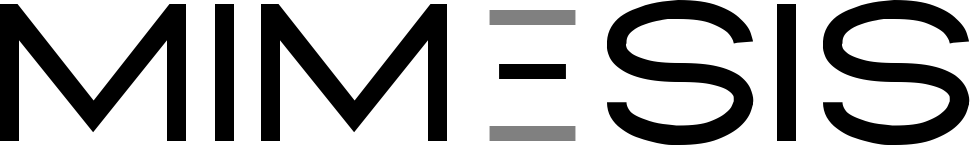
\includegraphics[width=0.2\textwidth]{mimesis.png}
\end{tcolorbox}
}


% Insert here the info that will be displayed into your Title page
% -> title of your work
% -> author name and surname
% -> MSc course
\newcommand\norm[1]{\lVert#1\rVert}





%------------------------------------------------------------------------------
%	TITLE PAGE

%------------------------------------------------------------------------------
\title{A mathematical model for Alzheimer's disease:}
\subtitle{from a microscopic to a macroscopic model using the Two-Scale \\Homogenization Theory}
\author{Andrea Bonifacio}

\date{}


\begin{document}

\begin{frame}[plain]
\titlepage
\end{frame}

%------------------------------------------------------------------------------
%	PRESENTATION SLIDES
%------------------------------------------------------------------------------

%------------------------------------------------
\section{Introduction}
%------------------------------------------------
\begin{frame}
\frametitle{A brief introduction to Alzheimer's disease}
\begin{itemize}
\item Alzheimer's disease (AD) is a neurodegenerative disease that usually starts slowly and progressively worsens. It is the most common form of senile dementia but the cause of it is still poorly understood.

\item Inside the brain exists a protein called $\beta$-peptide,which has a substantial role in the process of synaptic degeneration. This protein is produced in monomeric form by every healthy brain, but some problems arise when,  by unknown reasons (partially genetic), some neurons start to present an imbalance between production and clearance of $\mathrm{A} \beta$ amyloid during aging.

\end{itemize}
\end{frame}

%------------------------------------------------
\begin{frame}
\frametitle{The idea}
\begin{itemize}
\item Having a mathematical model for Alzheimer's disease is crucial because the highly toxic polymers involved in the disease have a short lifespan and cannot be easily studied experimentally. Therefore, a mathematical model provides the only means to investigate the behavior of amyloid in this context.
\item The modeling process carried out in this paper starts again from the Smoluchowski equation: a system of PDEs which describes the evolving densities of diffusing particles that coagulate in pairs. In this report it will be studied the application of the Smoluchowski equation to the description of agglomeration of $\mathrm{A} \beta$ peptide.
\end{itemize}
\end{frame}

%------------------------------------------------

\begin{frame}
\frametitle{The idea}
\begin{itemize}
\item The main objective is to derive a macroscopic model starting from a microscopic one.
\item In Bertsch et al. (2016) the authors present a model for the evolution of AD at a macroscopic scale and over the entire lifetime of the patient. In this case, the process of diffusion and aggregation of $\mathrm{A}\beta$ is modeled by a Smoluchowski system with a source term, coupled with a kinetic-type transport equation that keeps into account the spreading of the disease. Clearly, at this scale, neurons are no more visible so that they can be described mathematically as points.
\end{itemize}
\end{frame}

%------------------------------------------------

\begin{frame}
\frametitle{The problem}
\begin{itemize}
    \item Passing from the microscopic to the macroscopic scale is not trivial. It involves a sort of ``averaging process'' and it is done using a method called homogenization. It consists in performing the limits of the solutions of PDEs and finding the set of equations of which these limits are solutions.
    \item To do so, will be used the two-scale convergence theory, which is a powerful tool to pass from the microscopic to the macroscopic scale.
\end{itemize}
\end{frame}

%------------------------------------------------

\section{Smoluchowski equation}
%------------------------------------------------
\begin{frame}
\frametitle{The Smoluchowski equation}
The Smoluchowski equation is a system of PDEs which describes the evolving densities of diffusing particles that coagulate in pairs. It has been used to describe a lot of phenomena. In this case, it will be used to describe the agglomeration of $\mathrm{A} \beta$ peptide, starting from monomers.  

This phenomenon is called coalescence and can be written formally as 
\[
    P_i + P_j \rightarrow P_{i+j}
\]
which means that two polymers of length $i$ and $j$ coagulate to form a polymer of length $i+j$.
\end{frame}

\begin{frame}
\frametitle{The Smoluchowski equation}
Under the assumption that the aggregation of cluster is the result of only Brownian motion or diffusion, the equations can be written as:
\begin{equation}
    \pdev{u_i}{t}(t,x) - d_i \Delta_x u_i(t,x) = Q_i(u) \quad \text{in } [0,T] \times \Omega,
    \label{eq:smoluchowski}
\end{equation}
where \(u_i\) is the concentration of the cluster of length \(i\), \(d_i\) is the diffusion coefficient, \(\Omega\) is the domain of the system and \(Q_i(u)\) is the gain term minus the loss term which  are defined in this way:
\begin{equation*}
    \begin{aligned}
    &Q_{g, i}=\frac{1}{2} \sum_{j=1}^{i-1} a_{i-j, j} u_{i-j} u_{j}, \\
    &Q_{l, i}=u_{i} \sum_{j=1}^{\infty} a_{i, j} u_{j}.
    \end{aligned}
\end{equation*}
\end{frame}

\begin{frame}
\frametitle{The Smoluchowski equation}
\begin{equation*}
    \begin{aligned}
    &Q_{g, i}=\frac{1}{2} \sum_{j=1}^{i-1} a_{i-j, j} u_{i-j} u_{j}, \\
    &Q_{l, i}=u_{i} \sum_{j=1}^{\infty} a_{i, j} u_{j}.
    \end{aligned}
\end{equation*}
$Q_{g,i}$ describes the increasing of concentrations of the cluster of length $i$,
$Q_{l,i}$ describes the depletion of the polymers of size $i$.
An important role is played by the coagulation coefficients $a_{i-j,j}$ which describe a situation where a polymer of length $i-j$ coagulates with a polymer of length $j$ to form one of length $i$. These coefficients are symmetric, indeed $a_{i,j}=a_{j,i}$.
\end{frame}


%------------------------------------------------
\section{Mathematical model}
%------------------------------------------------
\subsection{Domain}
\begin{frame}
\frametitle{The domain}
\begin{columns}
    \column{0.5\textwidth}
    A piece of cerebral tissue is considered as the domain \(\Omega\). Inside this domain it is necessary to find a way to represent the presence of neurons, which is not so straightforward as it may seem. The idea is to represent the neurons as a set of holes in the domain. 
    \column{0.5\textwidth}
    \begin{figure}
        \centering
        {\incfig{domain_empty}}
        \caption{The domain \(\Omega\) representing the cerebral tissue.}
        \label{fig:perforated_domain}
      \end{figure}
\end{columns}
\end{frame}

\begin{frame}
\frametitle{The periodic neuron}
 \begin{columns}
    \column{0.7\textwidth}
    Let $Y$ be the unit periodicity cell $\left[0,1\left[{ }^{3}\right.\right.$ shown here.

    To represent the neurons, it is necessary to consider them as holes inside the cell.

    Denote by $T$ an open subset of $Y$ with a smooth boundary $\Gamma$, such that \(\overline{T} \subset \operatorname*{Int}(Y)\).
    
    Now call with $Y^{*}=Y \backslash T$ the material part, the ``solid part'' of the brain. 
    \column{0.3\textwidth}
    \begin{figure}
        \centering
        {\incfig{cell}}
        \caption{The periodic neuron}
        \label{fig:neuron}
      \end{figure}
 \end{columns}

\end{frame}

\begin{frame}
\frametitle{The periodic neuron}
\begin{itemize}
    \item The set $T$ represents a generic neuron, and $Y^{*}$ the supporting cerebral tissue.
    \item Define $\tau(\epsilon \overline{T})$ to be the set of all translated images $\epsilon \overline{T}$ of the form $\epsilon(k+\overline{T}), k \in \mathbb{Z}^{3}$.
    \item Now are defined both the cerebral tissue domain $\Omega$ and the set of all neurons \(\tau(\epsilon \overline(T))\), so it's possible to define the set of neurons inside the domain as 
    \[
        T_\epsilon \coloneqq \Omega \cap \tau(\epsilon \overline{T}).
    \]
\end{itemize}
\end{frame}


\begin{frame}
    \frametitle{The perforated domain}
    \begin{columns}
        \column{0.5\textwidth}
        Define the perforated domain \(\Omega_\epsilon\) as
        \[
            \Omega_\epsilon \coloneqq \Omega \backslash T_\epsilon.
        \]
        Ensure that there exists a ``security zone'' where the neurons cannot touch the boundary of \(\Omega\).
        \begin{equation}
        \exists \delta>0 : \operatorname*{dist}\left(\partial\Omega, T_{\epsilon}\right)\geq\delta.
        \label{eq:security_zone}
        \end{equation}
        \column{0.5\textwidth}
        \begin{figure}
            \centering
            {\incfig{domain}}
            \caption{The perforated domain \(\Omega_\epsilon\) representing the cerebral tissue full of neurons.}
            \label{fig:perforated_domain}
          \end{figure}
    \end{columns}
\end{frame}

\begin{frame}
    \frametitle{Boundaries}
    The boundaries of the domain are divided into two parts:
    \begin{itemize}
        \item $\partial{\Omega}$ is the boundary of the external domain \(\Omega\).
        \item $\Gamma_{\epsilon}$ is the boundary of the set of neurons \(T_{\epsilon}\) defined as
        \[
            \Gamma_{\epsilon} \coloneqq \bigcup\left\{\partial(\epsilon(k+\overline{T})) \mid \epsilon(k+\overline{T}) \subset \Omega\right\}.
        \]
        \item \(\partial\Omega_\epsilon \coloneqq \partial\Omega + \Gamma_\epsilon \).
    \end{itemize}
    \(\epsilon\) will denote the general term of a sequence of real numbers converging to zero.
\end{frame}

\subsection*{Equations}

\begin{frame}
    \frametitle{The Smoluchowski equation in the perforated domain}
   \begin{itemize}
    \item  Consider the vector-valued function $u=(u_1,\dots, u_M)$, where $u_j=u_j(t,x)$ $(t\geq 0, t\in \mathbb{R}$ and $x\in \Omega)$ is the molar concentration at the point $x$ and at the time $t$ of an assembly of $j$ monomers.
    \item With the definition of $u_M$ it is assumed that `large' assemblies do not aggregate to each other.
    \item The model is built assuming only binary coagulation.
   \end{itemize}
\end{frame}

\begin{frame}
    \frametitle{The Smoluchowski equation in the perforated domain}
    The model is given by a system of PDEs:
\begin{itemize}
    \item The first equation describes the evolution of monomers:
    \begin{equation}
        \begin{dcases}
        \begin{split}
            \frac{\partial u_{1}^{\epsilon}}{\partial t}(t, x)-d_{1} \Delta_{x} u_{1}^{\epsilon}(t, x) \\ 
            +u_{1}^{\epsilon}(t, x) \sum_{j=1}^{M} a_{1, j} u_{j}^{\epsilon}(t, x)=0,
        \end{split} & \text { in }[0, T] \times \Omega_{\epsilon},\\
        \frac{\partial u^{\epsilon}_1}{\partial v} \equiv \nabla_{x} u^{\epsilon}_1\cdot n=0, & \text { on }[0, T]\times\partial\Omega,\\
        \frac{\partial u^{\epsilon}_{1}}{\partial v} \equiv \nabla_{x} u^{\epsilon}_1 \cdot n=\epsilon \psi\left(t, x,\frac{x}{\epsilon}\right), & \text { on }[0, T] \times \Gamma_{\epsilon},\\
        u_{1}^{\epsilon}(0, x)=U_{1}, & \text{ in }\Omega_{\epsilon}.
        \end{dcases}
    \label{eq:u_1_eqs}\end{equation} 
\end{itemize}
\end{frame}

\begin{frame}
    \frametitle{The Smoluchowski equation in the perforated domain}
\begin{itemize}
    \item The second system of equation describes the evolution of the clusters with size \(1 < m < M\):
    \begin{equation}
        \begin{dcases}
           \begin{split}
             \frac{\partial u_{m}^{\epsilon}}{\partial t}(t, x)-d_{m} \Delta_{x} u_{m}^{\epsilon}(t, x) \\
            +u_{m}^{\epsilon}(t, x) \sum_{j=1}^{M} a_{m, j} u_{j}^{\epsilon}(t, x) \\
            = \frac{1}{2} \sum_{j=1}^{m-1} a_{j, m-j} u_{j}^{\epsilon} u_{m-j}^{\epsilon}
           \end{split}, & \text { in }[0, T] \times \Omega_{\epsilon},\\
            \frac{\partial u_{m}^{\epsilon}}{\partial v} \equiv \nabla_{x} u_{m}^{\epsilon} \cdot n=0,  & \text { on }[0, T]\times\partial\Omega_\epsilon, \\
         u_{m}^{\epsilon}(0, x)=0, & \text{ in } \Omega_{\epsilon}.
        \end{dcases}
    \label{eq:u_m_eqs}\end{equation}
\end{itemize}
\end{frame}

\begin{frame}
    \frametitle{The Smoluchowski equation in the perforated domain}
\begin{itemize}
    \item The last system of equation describes the evolution of the clusters with size \(M\):
    \begin{equation}
        \begin{dcases}
            \begin{split}
                \frac{\partial u_{M}^{\epsilon}}{\partial t}(t, x)-d_{M} \Delta_{x} u_{M}^{\epsilon}(t, x) \\
                = \frac{1}{2} \sum_{\mathclap{\substack{j+k\geq M\\j,k <M}}} a_{j, k} u_{j}^{\epsilon} u_{k}^{\epsilon}
            \end{split}, & \text { in }[0, T] \times \Omega_{\epsilon},\\
            \frac{\partial u_{M}^{\epsilon}}{\partial v} \equiv \nabla_{x} u_{M}^{\epsilon} \cdot n=0,  & \text { on }[0, T]\times\partial\Omega_\epsilon,
            \\
            u_{M}^{\epsilon}(0, x)=0, & \text{ in }\Omega_{\epsilon}.
        \end{dcases}
        \label{eq:u_M_eqs}
    \end{equation}
\end{itemize}
\end{frame}

\begin{frame}
    \frametitle{The Smoluchowski equation in the perforated domain}
    In \eqref{eq:u_1_eqs} $\epsilon$ is put in front of $\psi$ to prevent the divergence of the integral in a further passage, in order to avoid singularities. 
    The variable $x$ is called the slow scale variable, while the variable  $\frac{x}{\epsilon}$ is called the fast scale variable, which represents the microscopic scale.

    It's assumed that for $t>0$ the brain becomes sick. For technical reasons some regularity is needed on $\psi$ and $U_1$:
    \begin{enumerate}
        \item $\psi\left(t, x, \frac{x}{\epsilon}\right) \in C^{1}(0, T ; B)$ with $B=C^{1}\left[\bar{\Omega} ; C_{\text {\# }}^{1}(Y)\right]$, where $C_{\#}^{1}(Y)$ is the subset of $C^{1}\left(\mathbb{R}^{N}\right)$ of $Y$-periodic functions;
        \item $\psi\left(t=0, x, \frac{x}{\epsilon}\right)=0$
        \item 
    $U_{1}$ is a positive constant such that
    \begin{equation}
    U_{1} \leq\|\psi\|_{L^{\infty}(0, T ; B)} .
    \label{eq:U_1_norm}\end{equation}
    \end{enumerate}
\end{frame}

\begin{frame}
    \frametitle{Convergence to the macroscopic model}
    At this point the idea is to go from microscopic to macroscopic, by a sort of ``averaging process''. Indeed, the objective is to perform the homogenization on the set \eqref{eq:u_1_eqs}-\eqref{eq:u_m_eqs} of equations as $\epsilon \rightarrow 0$, however there is not a clear notion of convergence for the sequence $u_j^{\epsilon}$ $1\geq j \geq M$ which is defined on a varying set $\Omega_{\epsilon}$, which also is random perforated.
\end{frame}

\begin{frame}
    \frametitle{Convergence to the macroscopic model}
    \begin{theorem} 
    If $\epsilon>0$, the system \eqref{eq:u_1_eqs}-\eqref{eq:u_m_eqs} has a unique solution
    $$
    \left(u_{1}^{\epsilon}, \ldots, u_{M}^{\epsilon}\right) \in C^{1+\alpha / 2,2+\alpha}\left([0, T] \times \Omega_{\epsilon}\right) \quad(\alpha \in(0,1))
    $$
    such that
    $$
    u_{j}^{\epsilon}(t, x)>0 \text { for }(t, x) \in(0, T) \times \Omega_{\epsilon}, j=1, \ldots, M .
    $$
    \label{thm:3.1}
    \end{theorem}
\end{frame}




%------------------------------------------------------------------------------

\section{Two-scale convergence}

\begin{frame}
    \frametitle{Two-scale convergence definition}
    Two-scale convergence is a powerful tool that can help the study of functions in perforated domains. 
    \begin{definition}[Two-scale convergence]
        A sequence of functions $ v ^ {\epsilon } $in $ L^2([ 0 ,T]\times\Omega) $ two-scale converges to $v_{0} \in L^2([ 0 ,T]\times\Omega \times Y)$ if
        \begin{equation*}
        \begin{split}
            \lim_{\epsilon \to 0} \int_{0}^{\textrm{T}} \int_{\Omega} v^{\epsilon}(t,x)\psi\left(t,x,\frac{x}{\epsilon}\right) \, dxdt \\
            =\int_{0}^{\textrm{T}} \int_{\Omega} \int_{\textrm{Y}} v(t,x,y)\psi(t,x,y) \, dydxdt
        \end{split}
        \end{equation*}
 
        for all $\psi \in C^1([0,T]\times \bar\Omega;C_{\#}^{\infty}(Y))$
        \label{def 7.1}\end{definition}

\end{frame}


\begin{frame}
    \frametitle{Compactness theorem}
    This definition makes sense because of the next compactness theorem 
    \begin{theorem}[Compactness Theorem]
    If $v^{\epsilon}$ is a bounded sequence in $ L^2([ 0 ,T]\times\Omega) $, then there exist a function $v_{0}(t,x,y) \in   L^2([0,T]\times\Omega \times Y)$ s.t. $v^{\epsilon}$ two-scale converges to $v_{0}$, we write: 
    $v^{\epsilon} \overset{2s}{\rightharpoonup} v_{0}$.
    \label{thm 7.1}\end{theorem}
    This theorem is important because it shows that the minimal requirement to have two-scale convergence is that $v$ must be bounded.
    \end{frame}

\begin{frame}
    \frametitle{Relation with weak convergence}
    \begin{remark}[Remark, relation with weak convergence] If it is assumed that $\psi$ is independent of $y$, it will be obtained:
    \begin{equation*}
    \begin{split}
        \lim_{\epsilon \to 0} \int_{\Omega} v^{\epsilon}(x)\psi(x)dx 
        = \int_{\Omega} \int_{\textrm{Y}} v(x,y)\psi(x)dy \, dx \\
        =\int_{\Omega} \left[\int_{\textrm{Y}} v(x,y)dy\right]\psi(x)dx.
    \end{split}
    \end{equation*}
    This shows that, in this specific case, the two-scale convergence coincides with the weak convergence. Therefore, the two-scale convergence and the weak convergence are strictly related: the main difference between them is that in the first one the oscillations are captured due to the extra variable $y$.
    \end{remark}
\end{frame}

\begin{frame}[allowframebreaks]
    \frametitle{Two-scale convergence of products}
    The next theorems yield a characterization of the two-scale limit of the gradients of bounded sequences $v^{\epsilon}$ which is a critical result in order to apply the homogenization on problems. This theorem shows that, under specific hypotheses, the limit of the product coincides with the product of the limits.
    \begin{theorem}
    Let $v^{\epsilon}$ be a sequence of functions in $L^{2}([0, T] \times \Omega)$ which two-scale converges to a limit $v_{0} \in L^{2}([0, T] \times \Omega \times Y)$. Suppose, furthermore, that
    $$
    \lim _{\epsilon \rightarrow 0} \int_{0}^{T} \int_{\Omega}\left|v^{\epsilon}(t, x)\right|^{2} \, dxdt=\int_{0}^{T} \int_{\Omega} \int_{Y}\left|v_{0}(t, x, y)\right|^{2} \, dy dx dt.
    $$
    \theorembreak
    Then, for any sequence $w^{\epsilon}$ in $L^{2}([0, T] \times \Omega)$ that two-scale converges to a limit $w_{0} \in L^{2}([0, T] \times \Omega \times Y)$, we have
    $$
    \begin{aligned}
    \lim _{\epsilon \rightarrow 0} \int_{0}^{T} \int_{\Omega} v^{\epsilon}(t, x) & w^{\epsilon}(t, x) \phi\left(t, x, \frac{x}{\epsilon}\right) \, dxdt \\
    &=\int_{0}^{T} \int_{\Omega} \int_{Y} v_{0}(t, x, y) w_{0}(t, x, y) \phi(t, x, y) \, dy dx dt
    \end{aligned}
    $$for all $\phi \in C^{1}\left([0, T] \times \bar{\Omega} ; C_{\#}^{\infty}(Y)\right)$.
    \label{thm 7.2}\end{theorem}
\end{frame}

\begin{frame}
    \frametitle{Sobolev spaces}
    Here's a brief introduction to the Sobolev spaces, which can be ``improperly'' defined as \(L^p\) spaces with \(L^p\) derivatives. Formally
    \begin{definition}
        The Sobolev space $W^{1, p}(\Omega)$ is defined by
        $$
        W^{1, p}(\Omega)=\left\{v \mid v \in L^{p}(\Omega), \frac{\partial v}{\partial x_{i}} \in L^{p}(\Omega), i=1, \ldots, N\right\}
        $$
    \end{definition}
    Identify $H^{1}(\Omega)=W^{1,2}(\Omega)$, where and denote by $H_{\#}^{1}(Y)$ the closure of $C_{\#}^{\infty}(Y)$ for the $H^{1}$-norm.
    
    Now it's possible to introduce the next useful results.
\end{frame}

\begin{frame}[allowframebreaks]
    \frametitle{Managing gradients}
    When the limit is performed it appears an extra variable and one needs a theorem that defines how to manage the gradient of this variable.
\begin{theorem}
Let $v^{\epsilon}$ be a bounded sequence belonging in $L^{2}\left(0, T ; H^{1}(\Omega)\right)$ such that $v_{\epsilon}(t,x)\rightharpoonup v(t,x)$  in $L^{2}\left(0, T ; H^{1}(\Omega)\right)$. Then $v^{\epsilon} \overset{2s}{\rightharpoonup} v(t, x)$, and there exists a function $v_{1}(t, x, y)$ in $L^{2}\left([0, T] \times \Omega ; H_{\#}^{1}(Y) / \mathbb{R}\right)$ such that, up to a subsequence, $\nabla v^{\epsilon}  \overset{2s}{\rightharpoonup} \left(\nabla_{x} v(t, x)+\nabla_{y} v_{1}(t, x, y)\right)$. 
\label{thm 7.3}\end{theorem}
\begin{theorem} Let $v^{\epsilon}$ and $\epsilon \nabla v^{\epsilon}$ be two bounded sequences in $L^{2}([0, T] \times \Omega)$. Then, there exists a function $v_{1}(t, x, y)$ in $L^{2}\left([0, T] \times \Omega ; H_{\#}^{1}(Y) / \mathbb{R}\right)$ such that, up to a subsequence, $v^{\epsilon}$ and $\epsilon \nabla v^{\epsilon}$ two-scale converge to $v_{1}(t, x, y)$ and $\nabla_{y} v_{1}(t, x, y)$, respectively.
\label{theorem 7.4}\end{theorem}
\end{frame}


\begin{frame}[allowframebreaks]
    \frametitle{Generalization to the boundary}
    The main result of two-scale convergence can be generalized to the case of sequences defined on the boundary of the holes: $L^{2}\left([0, T] \times \Gamma_{\epsilon}\right)$.
    \begin{theorem}
    Let $v^{\epsilon}$ be a sequence in $L^{2}\left([0, T] \times \Gamma_{\epsilon}\right)$ such that
    $$
    \epsilon \int_{0}^{T} \int_{\Gamma_{\epsilon}}\left|v^{\epsilon}(t, x)\right|^{2} \, d\sigma_{\epsilon}(x)dt \leq C,
    $$
    where $C$ is a positive constant, independent of $\epsilon$.
    \theorembreak
    Then there exists a subsequence (still denoted by $\epsilon$) and a two-scale limit $v_{0}(t, x, y) \in L^{2}\left([0, T] \times \Omega ; L^{2}(\Gamma)\right)$ such that $v^{\epsilon}(t, x)$ two-scale converges to $v_{0}(t, x, y)$ in the sense that
    $$
    \begin{aligned}
    &\lim _{\epsilon \rightarrow 0} \epsilon \int_{0}^{T} \int_{\Gamma_{\epsilon}} v^{\epsilon}(t, x) \phi\left(t, x, \frac{x}{\epsilon}\right) \mathrm{d} t \mathrm{~d} \sigma_{\epsilon}(x) \\
    &=\int_{0}^{T} \int_{\Omega} \int_{\Gamma} v_{0}(t, x, y) \phi(t, x, y) \mathrm{d} t \mathrm{~d} x \mathrm{~d} \sigma(y)
    \end{aligned}
    $$
    for any function $\phi \in C^{1}\left([0, T] \times \bar{\Omega} ; C_{\#}^{\infty}(Y)\right)$.
    \label{thm 7.5}\end{theorem}
    
\end{frame}



%------------------------------------------------

\section{Homogenization of the Smoluchowsky equation}

\begin{frame}[allowframebreaks]
    \frametitle{Estimates on \(u_m^\epsilon, \nabla_x u_m^\epsilon\)}
    Since the homogenization will be carried out in the framework of two-scale convergence, the first necessary step is to obtain the a priori estimates for the sequences $u_{j}^{\epsilon}, \nabla u_{j}^{\epsilon}, \partial_{t} u_{j}^{\epsilon}$ in $[0, T] \times \Omega_{\epsilon}$. Here will be presented the estimate on the solution and its gradient.
    \begin{lemma} Let $T>0$ be arbitrary and $u_{1}^{\epsilon}$ be a classical solution of \eqref{eq:u_1_eqs}. Then,
    \begin{equation} \left\|u_{1}^{\epsilon}\right\|_{L^{\infty}\left(0, T ; L^{\infty}\left(\Omega_{\epsilon}\right)\right)} \leq\left|U_{1}\right|+\left\|u_{1}^{\epsilon}\right\|_{L^{\infty}\left(0, T ; L^{\infty}\left(\Gamma_{\epsilon}\right)\right)}. 
    \label{eq 20}\end{equation}
    \label{lemma 5.1}\end{lemma}
    \begin{lemma} Let $T>0$ be arbitrary and $u_{1}^{\epsilon}$ be a classical solution of \eqref{eq:u_1_eqs}. Then,
    \begin{equation}
        \left\|u_{1}^{\epsilon}\right\|_{L^{\infty}\left(0, T ; L^{\infty}\left(\Gamma_{\epsilon}\right)\right)} \leq c\|\psi\|_{L^{\infty}(0, T ; B)},
    \label{eq 21}\end{equation}where $c$ is independent of $\epsilon$.
    \label{lemma 5.2}\end{lemma}
    Thus, the boundedness of $u_{1}^{\epsilon}(t, x)$ in $L^{\infty}\left([0, T] \times \Gamma_{\epsilon}\right)$, uniformly in $\epsilon$, can be immediately deduced from Lemma \eqref{lemma 5.2} applying Lemma \eqref{lemma 5.1}.
    \begin{lemma}
    The sequence $\nabla_{x} u_{1}^{\epsilon}$ is bounded in $L^{2}\left([0, T] \times \Omega_{\epsilon}\right)$, uniformly in $\epsilon$.
      \label{lemma 5.4}\end{lemma}
    The lemmas considered show the boundedness of the term $u_1^{\epsilon}(t,x)$ and $\nabla_{x} u_{1}^{\epsilon}(t, x)$. With a similar procedure one can show the boundedness of the generic term $u_m$ and of its gradient.
\end{frame}

\begin{frame}
    \frametitle{Estimate on \(\partial u_m^\epsilon\)}
    \begin{lemma} The sequence $\partial_{t} u_{j}^{\epsilon}(1 \leq j \leq M)$ is bounded in $L^{2}\left([0, T] \times \Omega_{\epsilon}\right)$, uniformly in $\epsilon$.
        \label{lemma 5.9}
    \end{lemma}
\end{frame}
        
\begin{frame}
    \frametitle{Estimate on \(\partial u_m^\epsilon\)}
    \begin{proofs}
        Case $j=1$: multiply the first equation in \eqref{eq:u_1_eqs} by the function $\partial_{t} u_{1}^{\epsilon}(t, x)$. By the divergence theorem, by Hölder's and Young's inequalities, following the same arguments of the previous proofs and exploiting the boundedness of $u_{j}^{\epsilon}(t, x)(1 \leq j \leq M)$ in $L^{\infty}\left(0, T ; L^{\infty}\left(\Omega_{\epsilon}\right)\right)$, one can get
        \begin{equation}
         \begin{split}
             \int_{\Omega_{\epsilon}}\left|\frac{\partial u_{1}^{\epsilon}}{\partial t}\right|^{2} \, d  x+d_{1} \frac{\partial}{\partial t} \int_{\Omega_{\epsilon}}\left|\nabla_{x} u_{1}^{\epsilon}\right|^{2} \, d  x \\
             \leq C_{1}+2 \epsilon d_{1} \int_{\Gamma_{\epsilon}} \psi\left(t, x, \frac{x}{\epsilon}\right) \frac{\partial u_{1}^{\epsilon}}{\partial t} \, d  \sigma_{\epsilon}(x).
         \end{split}
        \label{eq 78}\end{equation}
    \end{proofs}
\end{frame}
\begin{frame}
    \frametitle{Estimate on \(\partial u_m^\epsilon\)}
    \begin{proofc}
        Integrating over $[0, t]$ with $t \in[0, T]$, it is possible to obtain
        \begin{equation}
            \begin{split}
                \int_{0}^{t} \, d  s \int_{\Omega_{\epsilon}}\left|\frac{\partial u_{1}^{\epsilon}}{\partial s}\right|^{2} \, d   x+d_{1}\left(1-\epsilon^{2} C_{3}\right) \int_{\Omega_{\epsilon}}\left|\nabla_{x} u_{1}^{\epsilon}\right|^{2} \, d  x \\
                 \leq C_{1} T+C_{4}+C_{7},
            \end{split}
          \label{eq 80}\end{equation}
          where the positive constants $C_{1}, C_{3}, C_{4}, C_{7}$ are independent of $\epsilon$, since $\psi \in$ $L^{\infty}(0, T ; B), u_{1}^{\epsilon}$ is bounded in $L^{\infty}\left(0, T ; L^{\infty}\left(\Omega_{\epsilon}\right)\right), \nabla_{x} u_{1}^{\epsilon}$ is bounded in $L^{2}(0, T$; $L^{2}\left(\Omega_{\epsilon}\right)$) and the following inequality holds
    \end{proofc}
\end{frame}
\begin{frame}
    \frametitle{Estimate on \(\partial u_m^\epsilon\)}
    \begin{proofe}
        $$
        \epsilon \int_{\Gamma_{\epsilon}}\left|\partial_{t} \psi\left(t, x, \frac{x}{\epsilon}\right)\right|^{2} \, d  \sigma_{\epsilon}(x) \leq \tilde{C}\left\|\partial_{t} \psi(t)\right\|_{B}^{2} \leq C_{5}
        $$
        with $\tilde{C}$ and $C_{5}$ independent of $\epsilon$. For a sequence $\epsilon$ of positive numbers going to zero: $\left(1-\epsilon^{2} C_{3}\right) \geq 0$. Then, the second term on the left-hand side of \eqref{eq 80} is nonnegative, and one has
        \begin{equation}
          \left\|\partial_{t} u_{1}^{\epsilon}\right\|_{L^{2}\left(0, T ; L^{2}\left(\Omega_{\epsilon}\right)\right)}^{2} \leq C,
        \label{eq 81}\end{equation}
        where $C \geq 0$ is a constant independent of $\epsilon$.
        A similar procedure can be applied to the generic term $u_m$.
    \end{proofe}
\end{frame}

\begin{frame}[allowframebreaks]
    \frametitle{Extension lemma}
    The proofs of the previous Lemmas rely on a generalization to perforated domains of the main inequalities valid in \(\Omega\), through the following extension Lemma:
    \begin{lemma}
  
        Suppose that the domain $\Omega_{\epsilon}$ is such that assumption \eqref{eq:security_zone} is satisfied. Then, there exists a family of linear continuous extension operators
       
       $$
       P_{\epsilon}: W^{1, p}\left(\Omega_{\epsilon}\right) \rightarrow W^{1, p}(\Omega)
       $$
       \theorembreak 
        and a constant $C>0$ independent of $\epsilon$ such that
       
       $$
       P_{\epsilon} v=v \quad \text { in } \Omega_{\epsilon}
       $$
       and
       \begin{equation}
         \int_{\Omega}\left|P_{\epsilon} v\right|^{p} \, d  x \leq C \int_{\Omega_{\epsilon}}|v|^{p} \, d  x,
       \label{eq 114}\end{equation}
       \begin{equation}
         \int_{\Omega}\left|\nabla\left(P_{\epsilon} v\right)\right|^{p} \, d  x \leq C \int_{\Omega_{\epsilon}}|\nabla v|^{p} \, d  x
       \label{eq 115}\end{equation}
       
       for each $v \in W^{1, p}\left(\Omega_{\epsilon}\right)$ and for any $p \in(1,+\infty)$.
       \label{lemma 7.2}\end{lemma}
\end{frame}

%------------------------------------------------

\section{Main theorem}

\begin{frame}[allowframebreaks]
    \frametitle{Statement of the main theorem}
        \begin{itemize}
        \item     Now that all the necessary result are obtained, it's possible to state the main theorem of the homogenization of the Smoluchowski equation in perforated domains.
        \item Theorem \eqref{thm 5.1} shows that the macroscale (homogenized) model, obtained from Eqs. \eqref{eq:u_1_eqs}-\eqref{eq:u_M_eqs} as $\epsilon \rightarrow 0$, is asymptotically consistent with the original model and resolves both the coarse and the small scale. 
        \item The information given on the microscale, by the non-homogeneous Neumann boundary condition in \eqref{eq:u_1_eqs}, is transferred into the source term in the first equation of \eqref{eq 16}, describing the limit model. 
        \end{itemize}

    \begin{theorem} Let $u_{m}^{\epsilon}(t, x)(1 \leq m \leq M)$ be a family of classical solutions to problems \eqref{eq:u_1_eqs}-\eqref{eq:u_M_eqs}. The sequences $\widetilde{u_{m}^{\epsilon}}$ and $\widetilde{\nabla_{x} u_{m}^{\epsilon}}(1 \leq m \leq M)$ two-scale converge to: $\left[\chi(y) u_{m}(t, x)\right]$ and $\left[\chi(y)\left(\nabla_{x} u_{m}(t, x)+\nabla_{y} u_{m}^{1}(t, x, y)\right)\right](1 \leq m \leq M)$, respectively, where tilde denotes the extension by zero outside $\Omega_{\epsilon}$ and $\chi(y)$ represents the characteristic function of $Y^{*}$. 
        The limiting functions $\left(u_{m}(t, x), u_{m}^{1}(t, x, y)\right)(1 \leq m \leq M)$ are the unique solutions in $L^{2}\left(0, T ; H^{1}(\Omega)\right) \times L^{2}\left([0, T] \times \Omega ; H_{\#}^{1}(Y) / \mathbb{R}\right)$ of the following two-scale homogenized systems.
        \label{thm 5.1}
    \end{theorem}
    \begin{block}{}
        If $m=1$:
        \begin{equation}
          \begin{dcases}
           \begin{split}
             \theta \frac{\partial u_{1}}{\partial t}(t, x)-\operatorname{div}_{x}\left[d_{1} A \nabla_{x} u_{1}(t, x)\right] \\  +\theta u_{1}(t, x) \sum_{j=1}^{M} a_{1, j} u_{j}(t, x) \\ =d_{1} \int_{\Gamma} \psi(t, x, y) \, d  \sigma(y), 
           \end{split} & \text { in }[0, T]\times\Omega, \\
            {\left[A \nabla_{x} u_{1}(t, x)\right] \cdot n=0}, & \text { on }[0, T]\times\partial\Omega, \\ 
            u_{1}(0, x)=U_{1}, & \text { in }\Omega. \\ 
        \end{dcases}
        \label{eq 16}
        \end{equation}
    \end{block}
    \begin{block}{}
        If $1<m<M$:
        \begin{equation}
          \begin{dcases}
            \begin{split}
                \theta \frac{\partial u_{m}}{\partial t}(t, x)-\operatorname{div}_{x}\left[d_{m} A \nabla_{x} u_{m}(t, x)\right] \\ +\theta u_{m}(t, x) \sum_{j=1}^{M} a_{m, j} u_{j}(t, x) & \\ =\frac{\theta}{2} \sum_{j=1}^{m-1} a_{j, m-j} u_{j}(t, x) u_{m-j}(t, x), 
            \end{split}& \text { in }[0, T]\times\Omega,\\ 
            {\left[A \nabla_{x} u_{m}(t, x)\right] \cdot n=0}, & \text { on }[0, T]\times\partial\Omega, \\ 
            u_{m}(0, x)=0, & \text { in }\Omega.
        \end{dcases}
        \label{eq 17}\end{equation}
    \end{block}
    \begin{block}{}
            If $m=M$:
            \begin{equation}
              \begin{dcases}
                \begin{split}
                    \theta \frac{\partial u_{M}}{\partial t}(t, x)-d i v_{x}\left[d_{M} A \nabla_{x} u_{M}(t, x)\right] & \\ =\frac{\theta}{2} \sum_{\substack{j+k \geq M \\ j,k<M}} a_{j, k} u_{j}(t, x) u_{k}(t, x),
                \end{split} & \text { in }[0, T]\times\Omega,\\ 
                {\left[A \nabla_{x} u_{M}(t, x)\right] \cdot n=0}, & \text { on }[0, T]\times\partial\Omega, \\ 
                u_{M}(0, x)=0,& \text { in }\Omega.
            \end{dcases}
            \label{eq 18}\end{equation}
            where
            $
            u_{m}^{1}(t, x, y) =\sum_{i=1}^{N} w_{i}(y) \frac{\partial u_{m}}{\partial x_{i}}(t, x) \quad(1 \leq m \leq M), 
            $
    \end{block}
    \begin{block}{}
            and
            $
            \theta =\int_{Y} \chi(y) \, d  y=\left|Y^{*}\right|
            $
            is the volume fraction of material, and $A$ is a matrix with constant coefficients defined by
                \begin{equation*}
                A_{i j}=\int_{Y^{*}}\left(\nabla_{y} w_{i}+\hat{e}_{i}\right) \cdot\left(\nabla_{y} w_{j}+\hat{e}_{j}\right) \, d  y,
                \end{equation*}
                with  $\hat{e}_{i}$ being the $ith$ unit vector in $\mathbb{R}^n$ and $(w_i)_1\leq i \leq N$ the family of solutions of the cell problem
                \begin{equation}
                    \begin{dcases}
                        -\operatorname{div}_{y}\left[\nabla_{y} w_{i}+\hat{e}_{i}\right]=0, & \text { in } Y^{*}, \\
                        \left(\nabla_{y} w_{i}+\hat{e}_{i}\right) \cdot n=0, & \text { on } \Gamma, \\
                        y \rightarrow w_{i}(y), & Y-\text {periodic}.
                    \end{dcases}
                    \label{eq 19}
                \end{equation}
        \end{block}
\end{frame}
\begin{frame}{Proof for \(m=1\) I}
    \begin{proofs}
        In view of Lemmas \eqref{lemma 5.1}-\eqref{lemma 5.2} and \eqref{lemma 5.4}, the sequences $\widetilde{u_{m}^{\epsilon}}$ and $\widetilde{\nabla_{x} u_{m}^{\epsilon}}(1 \leq m \leq M)$ are bounded in $L^{2}([0, T] \times \Omega)$, and by application of Theorem \eqref{thm 7.1} and Theorem \eqref{thm 7.3}, and so:
        \begin{equation}
        \widetilde{u_{m}^{\epsilon}}  \overset{2s}{\rightharpoonup}
        \left[\chi(y) u_{m}(t, x)\right],
        \end{equation}
        \begin{equation}
        \widetilde{\nabla_{x} u_{m}^{\epsilon}}
        \overset{2s}{\rightharpoonup}
        \left[\chi(y)\left(\nabla_{x} u_{m}(t, x)+\right.\right.\left.\left.\nabla_{y} u_{m}^{1}(t, x, y)\right)\right], \quad (1 \leq m \leq M).
        \end{equation}
    \end{proofs}
\end{frame}
\begin{frame}{Proof for \(m=1\) II}
    \begin{proofc}
        Similarly, in view of Lemma \eqref{lemma 5.9}, it is possible to prove that
        \begin{equation}
        \left(\widetilde{\frac{\partial u_{m}^{\epsilon}}{\partial t}}\right)
        \overset{2s}{\rightharpoonup}
        \left[\chi(y) \frac{\partial u_{m}}{\partial t}(t, x)\right],  \quad (1 \leq m \leq M).
        \end{equation}
        One can now find the homogenized equations satisfied by $u_{m}(t, x)$ and $u_{m}^{1}(t, x, y)$ $(1 \leq m \leq M)$.
        In the case $m=1$, multiply the first equation of \eqref{eq:u_1_eqs} by the test function to obtain the weak formulation of the problem
        $$
        \phi_{\epsilon} \equiv \phi(t, x)+\epsilon \phi_{1}\left(t, x, \frac{x}{\epsilon}\right),
        $$
    \end{proofc}
\end{frame}
\begin{frame}{Proof for \(m=1\) III}
    \begin{proofc}
        where $\phi \in C^{1}([0, T] \times \bar{\Omega})$ and $\phi_{1} \in C^{1}\left([0, T] \times \bar{\Omega} ; C_{\#}^{\infty}(Y)\right)$. 
        \begin{equation*}
            \frac{\partial u_{1}^{\epsilon}}{\partial t}\phi_{\epsilon}-\operatorname{div}\left(d_{1} \nabla_{x} u_{1}^{\epsilon}\right)\phi_{\epsilon}+u_{1}^{\epsilon} \sum_{j=1}^{M} a_{1, j} u_{1}^{\epsilon}\phi_{\epsilon}=0.
        \end{equation*}
    \end{proofc}
\end{frame}
\begin{frame}{Proof for \(m=1\) IV}
    \begin{proofc}
        Integrating, the divergence theorem yields
        \begin{equation}
          \begin{aligned}
        &\int_{0}^{T} \int_{\Omega_{\epsilon}} \frac{\partial u_{1}^{\epsilon}}{\partial t} \phi_{\epsilon}\left(t, x, \frac{x}{\epsilon}\right) \, d  t \, d  x\\ 
        &+d_{1} \int_{0}^{T} \int_{\Omega_{\epsilon}} \nabla_{x} u_{1}^{\epsilon} \cdot \nabla \phi_{\epsilon} \, d  t \, d  x \\
        &+\int_{0}^{T} \int_{\Omega_{\epsilon}} u_{1}^{\epsilon} \sum_{j=1}^{M} a_{1, j} u_{j}^{\epsilon} \phi_{\epsilon} \, d  t \, d  x\\
        &=\epsilon d_{1} \int_{0}^{T} \int_{\Gamma_{\epsilon}} \psi\left(t, x, \frac{x}{\epsilon}\right) \phi_{\epsilon} \, d  t \, d  \sigma_{\epsilon}(x).
        \end{aligned}
        \label{eq 86}\end{equation}
    \end{proofc}
\end{frame}
\begin{frame}{Proof for \(m=1\) V}
    \begin{proofc}
        Passing to the two-scale limit, one can get
        \begin{equation}
        \begin{aligned}
        &\int_{0}^{T} \int_{\Omega} \int_{Y^{*}} \frac{\partial u_{1}}{\partial t}(t, x) \phi(t, x) \, d  t \, d  x \, d  y \\
        &\quad+d_{1} \int_{0}^{T} \int_{\Omega} \int_{Y^{*}}\left[\nabla_{x} u_{1}(t, x)\right.+\\
        &\qquad \qquad \nabla_{y} u_{1}^{1}\left.(t, x, y)\right] \cdot\left[\nabla_{x} \phi(t, x)+\nabla_{y} \phi_{1}(t, x, y)\right] \, d  t \, d  x \, d  y\\
        &+\int_{0}^{T} \int_{\Omega} \int_{Y^{*}} u_{1}(t, x) \sum_{j=1}^{M} a_{1, j} u_{j}(t, x) \phi(t, x) \, d  t \, d  x \, d  y\\
        &= d_{1} \int_{0}^{T} \int_{\Omega} \int_{\Gamma} \psi(t, x, y) \phi(t, x) \, d  t \, d  x \, d  \sigma(y).
        \end{aligned}
        \label{eq 87}\end{equation}
    \end{proofc}
\end{frame}
\begin{frame}{Proof for \(m=1\) VI}
    \begin{proofc}
        The last term on the left-hand side of \eqref{eq 87} has been obtained by using Theorem \eqref{thm 7.2}, while the term on the right-hand side has been attained by application of Theorem \eqref{thm 7.5}. An integration by parts shows that \eqref{eq 87} is a variational formulation associated with the following homogenized system:
    \end{proofc}
\end{frame}
\begin{frame}{Proof for \(m=1\) VII}
    \begin{proofc}
        \begin{align}
        &\begin{split}
            -\operatorname{div}_{y}\left[d_{1}\left(\nabla_{x} u_{1}(t, x)+\nabla_{y} u_{1}^{1}(t, x, y)\right)\right]=0, \\
             \quad \text { in }[0, T] \times \Omega \times Y^{*},
        \end{split}\label{eq 88}\\
        &\begin{split}
            \left[\nabla_{x} u_{1}(t, x)+\nabla_{y} u_{1}^{1}(t, x, y)\right] \cdot n=0,\\
             \quad \text { on }[0, T] \times \Omega \times \Gamma,
        \end{split} \label{eq 89}
    \end{align}
\end{proofc}
\end{frame}
\begin{frame}{Proof for \(m=1\) VIII}
    \begin{proofc}
        \begin{flalign}
            &\begin{split}
            \theta \frac{\partial u_{1}}{\partial t}(t, x)-\operatorname{div}_{x}\left[d_{1} \int_{Y^{*}}\left(\nabla_{x} u_{1}(t, x)+\nabla_{y} u_{1}^{1}(t, x, y)\right) \, d  y\right] \\
            +\theta u_{1}(t, x) \sum_{j=1}^{M} a_{1, j} u_{j}(t, x)-d_{1} \int_{\Gamma} \psi(t, x, y) \, d  \sigma(y)=0,\\
            \quad \text { in }[0, T] \times \Omega,
            \end{split}
            \label{eq 90}\\
            &\begin{split}
                \left[\int_{Y^{*}}\left(\nabla_{x} u_{1}(t, x)+\nabla_{y} u_{1}^{1}(t, x, y)\right) \, d  y\right] \cdot n=0,\\
                 \quad \text { on }[0, T] \times \partial \Omega.
            \end{split}
            \label{eq 91}
        \end{flalign}
    \end{proofc}
\end{frame}
\begin{frame}{Proof for \(m=1\) IX}
    \begin{proofc}
        To conclude, by continuity, one can have that
        $$
        u_{1}(0, x)=U_{1} \quad \text { in } \Omega .
        $$
        Taking advantage of the constancy of the diffusion coefficient $d_{1}$, Eqs. \eqref{eq 88} and \eqref{eq 89} can be rewritten as follows
        \begin{equation}
        \Delta_{y} u_{1}^{1}(t, x, y)=0, \quad \text { in }[0, T] \times \Omega \times Y^{*},
        \label{eq 92}\end{equation}
        \begin{equation}
         \nabla_{y} u_{1}^{1}(t, x, y) \cdot n=-\nabla_{x} u_{1}(t, x) \cdot n, \quad \text { on }[0, T] \times \Omega \times \Gamma.
        \label{eq 93}\end{equation}
        \end{proofc}
\end{frame}
\begin{frame}{Proof for \(m=1\) X}
    \begin{proofc}
        Then, $u_{1}^{1}(t, x, y)$ satisfying (92)-(93) can be written as
        \begin{equation}
         u_{1}^{1}(t, x, y)=\sum_{i=1}^{N} w_{i}(y) \frac{\partial u_{1}}{\partial x_{i}}(t, x),
        \label{eq 94}\end{equation}
        where $\left(w_{i}\right)_{1 \leq i \leq N}$ is the family of solutions of the cell problem
        \begin{equation}
         \begin{cases}-\operatorname{div}_{y}\left[\nabla_{y} w_{i}+\hat{e}_{i}\right]=0, & \text { in } Y^{*}, \\ \left(\nabla_{y} w_{i}+\hat{e}_{i}\right) \cdot n=0, & \text { on } \Gamma, \\ y \rightarrow w_{i}(y), & Y-\text {periodic}. \end{cases}
        \label{eq 95}\end{equation}
    \end{proofc}
\end{frame}
\begin{frame}{Proof for \(m=1\) XI}
    \begin{proofc}
        By using the relation \eqref{eq 94} in Eqs. \eqref{eq 90} and \eqref{eq 91}, it is possible to get
        \begin{equation}
         \begin{split}
            \theta \frac{\partial u_{1}}{\partial t}(t, x)-\operatorname{div}_{x}\left[d_{1} A \nabla_{x} u_{1}(t, x)\right]+\theta u_{1}(t, x) \sum_{j=1}^{M} a_{1, j} u_{j}(t, x) \\
           -d_{1} \int_{\Gamma} \psi(t, x, y) \, d  \sigma(y)=0, \quad \text { in }[0, T] \times \Omega,
         \end{split}
        \label{eq 96}\end{equation}
        \begin{equation}
         \left[A \nabla_{x} u_{1}(t, x)\right] \cdot n=0, \quad \text { on }[0, T] \times \partial \Omega,
        \label{eq 97}\end{equation}
    \end{proofc}
\end{frame}
\begin{frame}{Proof for \(m=1\) XII}
    \begin{proofe}
        where $A$ is a matrix with constant coefficients defined by
        $$
        A_{i j}=\int_{Y^{*}}\left(\nabla_{y} w_{i}+\hat{e}_{i}\right) \cdot\left(\nabla_{y} w_{j}+\hat{e}_{j}\right) \, d  y .
        $$
        \end{proofe}
\end{frame}

%------------------------------------------------

\section{Conclusions}   

\begin{frame}
    \frametitle{Conclusions}
    \begin{itemize}
        \item The model presented here can be related to the one introduced in Bertsch et. al. (2016), where the process of diffusion and agglomeration of $\mathrm{A} \beta$ is described on the macroscale by a Smoluchowski system with a source term. 
        \item Performed a formal derivation, starting from the microscale, of the source term $\mathcal{F}$.
        \item It's good to notice that the homogenization theory works in every perforated domain so one can follow the previous arguments to homogenize every system in a random perforated domain.
    \end{itemize}
\end{frame}
% %------------------------------------------------------------------------------
%	TOC
%------------------------------------------------------------------------------



\end{document}